\chapter{Evaluation}
\label{chap:Evaluation}

Within this section, the evaluation process of this project will be outline, as well as the resulting experimental results.

Evaluating this swarm system successfully poses several questions:-

\begin{enumerate}
	\item Can the system be described as exhibiting flocking behaviour in line with the definition of a swarm system?
	\item How quickly does the system form a state of flocking?
	\item Does the swarm have the ability to form splinter groups?
	\item Can these splinter groups amalgamate to form one flock?
	\item How well does the system deal with failure?
	\item Is the swarm system scalable?
\end{enumerate}

Answering these questions will provide a thorough evaluation of the system's success. To that end, an experiment will be conducted for each question, with the aim of gathering data to make conclusions.
\clearpage

\section{Testing}

\subsubsection{Experiment 1: Can the system be described as exhibiting flocking behaviour in line with the definition of a swarm system?}

With regard to robotics, \citeauthor{VanDykeParunak2004} defined swarming as ``useful self-organization of multiple entities through local interactions''. \cite{VanDykeParunak2004} Following this definition, an assessment of the system can be made.

The ability of the system to self-organise and move as a group can be tested by executing the program and observing the simulation. The cohesiveness of the swarm can be validated by capturing both the GPS data and the number of detected robots in the swarm and comparing these.

The swarm may be evaluated further by comparing the behaviour of the system to the behaviour exhibited by natural systems and observing the similarities and differences.

\subsubsection{Experiment 2: How quickly does the system form a state of flocking?}

This can be measured by recording the current heading of the robot and the number of neighbours each robot detects, at every simulation time step. Once this data has been gathered, an analysis can be made.

\subsubsection{Experiment 3: Does the swarm have the ability to form splinter groups?}

This question can be answered by executing a simulation where some members of the swarm are segregated from the others and observing the behaviour over time. Also, positional and neighbourhood data can be gathered to further validate the conclusion.

\subsubsection{Experiment 3: Can these splinter groups amalgamate to form one flock?}

This question and the last can be tested during the same experiment. Once separate groups have been formed, the segregation can be removed and the behaviour of the two groups analysed.

\subsubsection{Experiment 4: How well does the system deal with failure?}

Failure within a swarm can be defined in a number of ways. The main point of failure, however, are the agents themselves. In this case it can be simulated by powering down robots during execution of the program. This will test to see if the system can adapt to changing circumstances. 

\subsubsection{Experiment 5: Is the swarm system scalable?}

One of the defining features of a robot swarm is the system's scalability. This can be easily tested through the addition of more agents to the swarm and observing the system's behaviour. GPS and neighbourhood data can also be gathered and these can be compared with different swarm sizes for analyses. 
\clearpage
\section{Results and Analysis}
\label{section:results}

Upon conducting the experiments outlined in the previous section, the results as well as a discussion of the findings are presented here.

\subsection{Experiment 1}

\begin{figure}[!h]
	\centering
	\begin{minipage}{.5\textwidth}
		\centering
		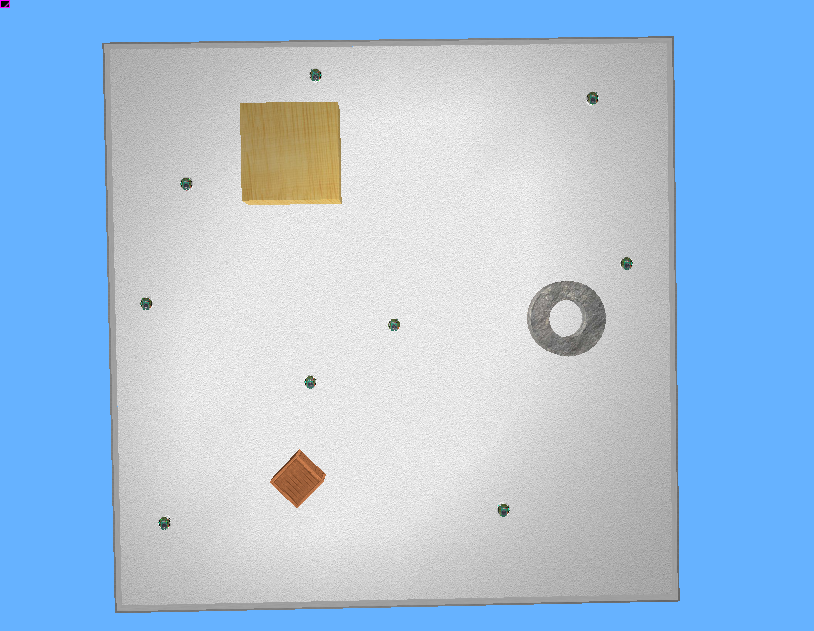
\includegraphics[width=.75\linewidth]{swarm_test_1}
		\caption*{t = 0s}
		\label{fig:sw1}
	\end{minipage}%
	\begin{minipage}{.5\textwidth}
		\centering
		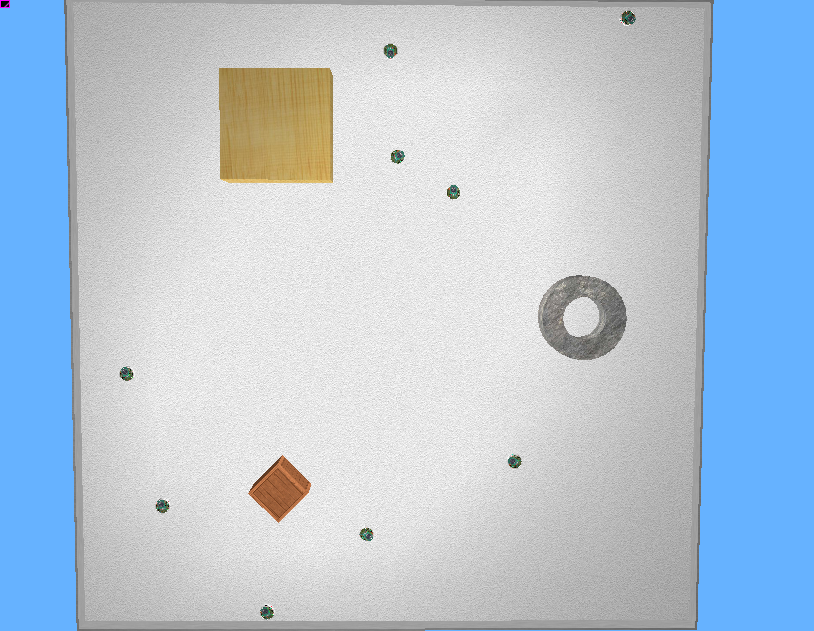
\includegraphics[width=.75\linewidth]{swarm_test_2}
		\caption*{t = 10s}
		\label{fig:sw2}
	\end{minipage}
	\begin{minipage}{.5\textwidth}
		\centering
		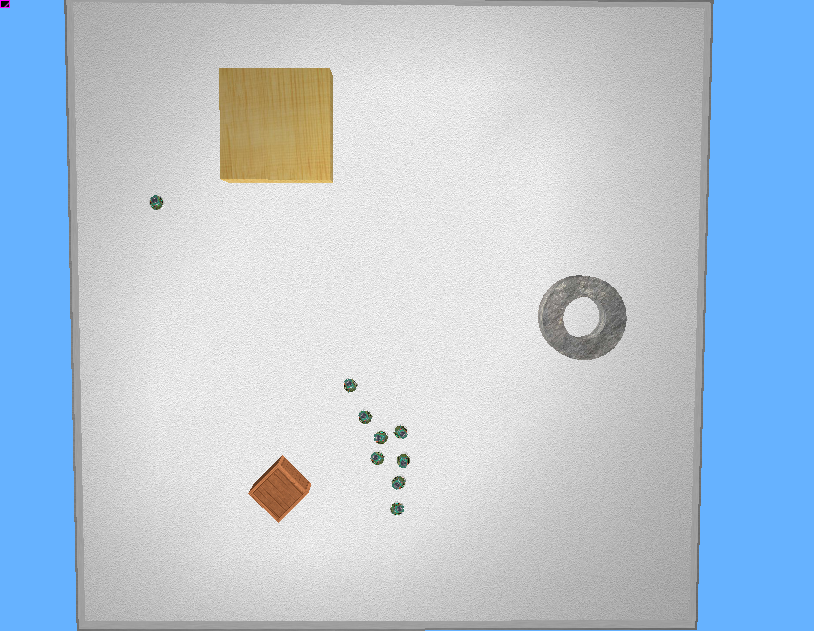
\includegraphics[width=.75\linewidth]{swarm_test_3}
		\caption*{t = 30s}
		\label{fig:sw3}
	\end{minipage}%
	\begin{minipage}{.5\textwidth}
		\centering
		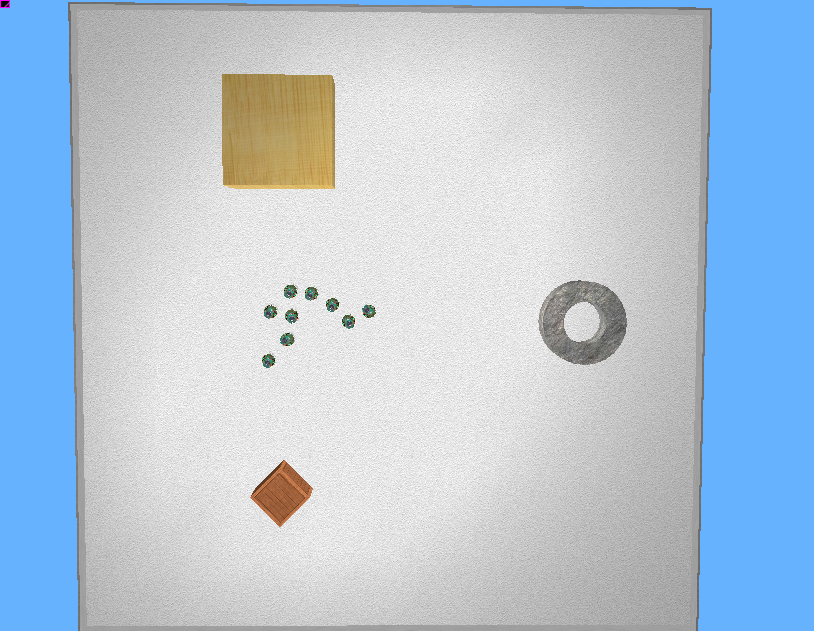
\includegraphics[width=.75\linewidth]{swarm_test_4}
		\caption*{t = 40s}
		\label{fig:sw4}
	\end{minipage}
		\captionof{figure}{Swarm movement over time}
		\label{fig:sw5}
\end{figure}

Figure \ref{fig:sw5} shows the movement of the swarm over a 40 second period. Initially, the robots are separated. As can be seen, at \(t = 10s\), each unit has moved relative to its starting position however do not yet exhibit group behaviour. Soon after this point though, the agents begin to coalesce into a cohesive group. By \(t = 30s\), the majority of agents are within detection range and are moving together. By \(t = 40s\), all of the agents have formed one group, which expand, contract and move around the environment together.

This can be shown graphically (Fig. \ref{fig:exp1}, Fig. \ref{fig:exp1-avg}), through the collection of data directly from the simulated robots. As can be seen, as time increases, the number of robots detected tends to the maximum in the arena.
\clearpage

\begin{sidewaysfigure}
	\centering
\begin{minipage}{1\textwidth}
	\centering
	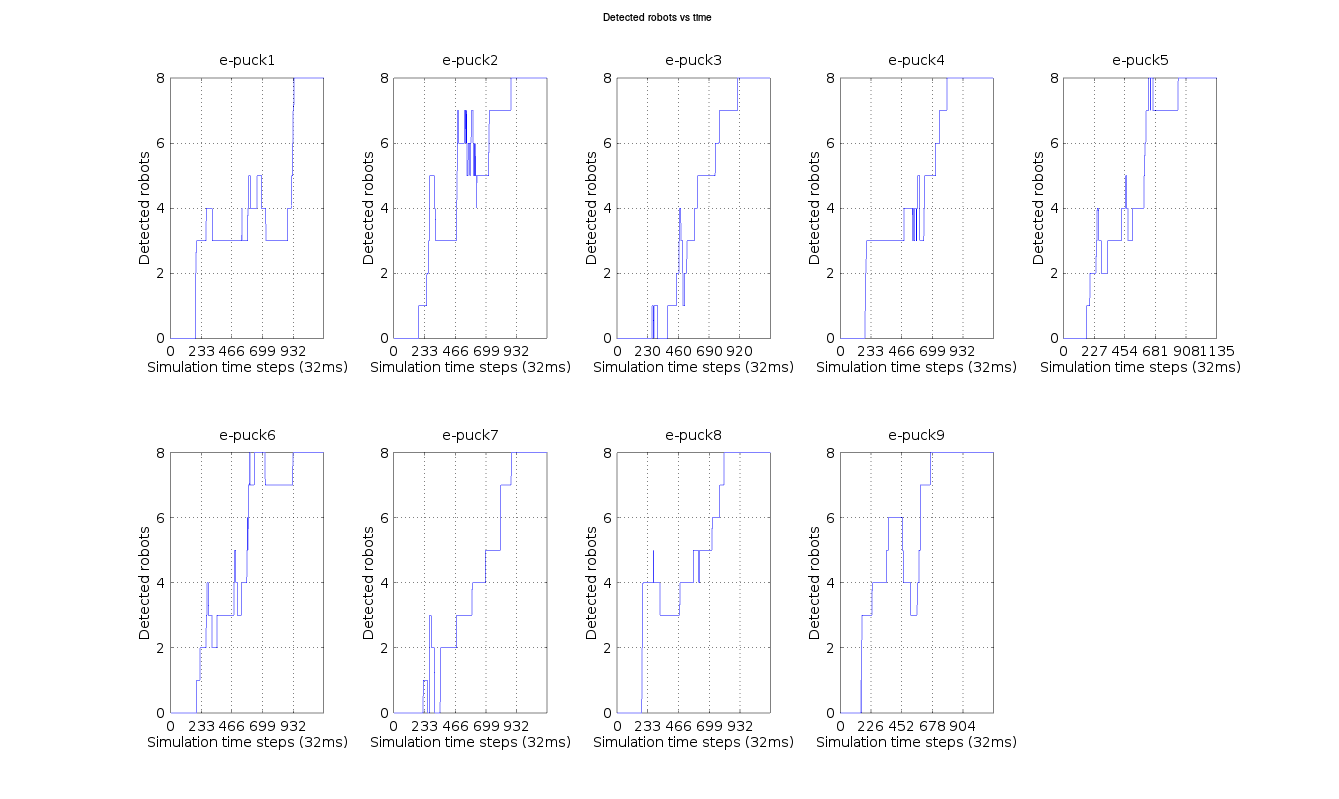
\includegraphics[width=1\linewidth]{data1}
	\captionof{figure}{Number of robots detected vs time}
	\label{fig:exp1}
\end{minipage}%
\end{sidewaysfigure}
\clearpage

\begin{figure}[!t]
		\centering
	\begin{minipage}{1\textwidth}
		\centering
		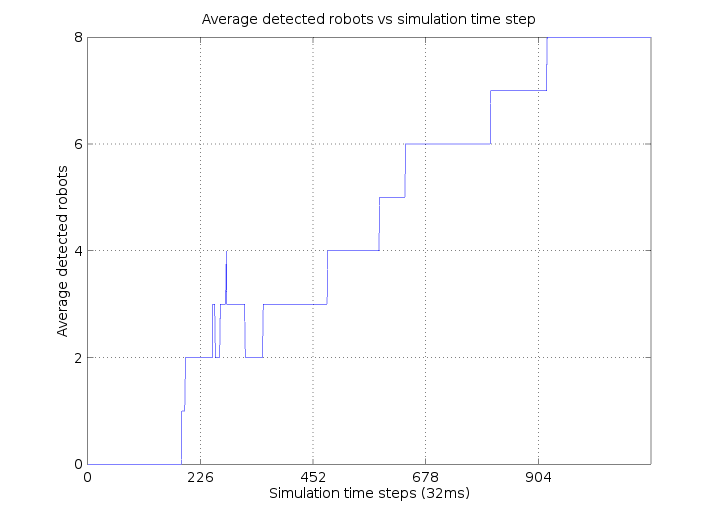
\includegraphics[width=1\linewidth]{data1-average}
		\captionof{figure}{Average number of detected robots}
		\label{fig:exp1-avg}
	\end{minipage}%
\end{figure}

This proves that given enough time, the swarm system will form into one cohesive flock. Due to the nature of the design of the system, there is no higher level supervisor (human or otherwise) co-ordinating the movements of the flock. Therefore, as the system moves to eventually form a group without external aid, the swarm can be said to exhibit self-organization. Furthermore, since each robot broadcasts information locally and does not require any form of positional data detailing the whole swarm, the system can be said to be only interacting locally.

Given the above analysis, this system satisfies \citeauthor{VanDykeParunak2004}'s definition of a swarm, \textit{``useful self-organization of multiple entities through local interactions''} \cite{VanDykeParunak2004}.

Next, the behavioural similarities to natural systems can be examined.

\clearpage

\begin{figure}[h]
	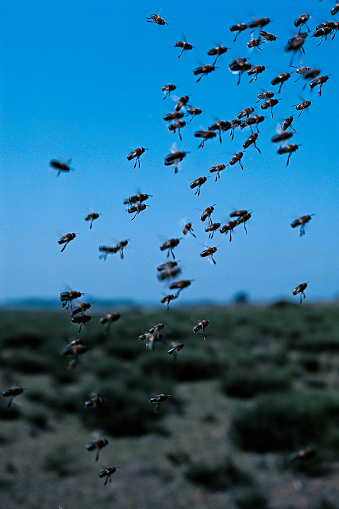
\includegraphics[width=.355\linewidth]{bee-swarm}
	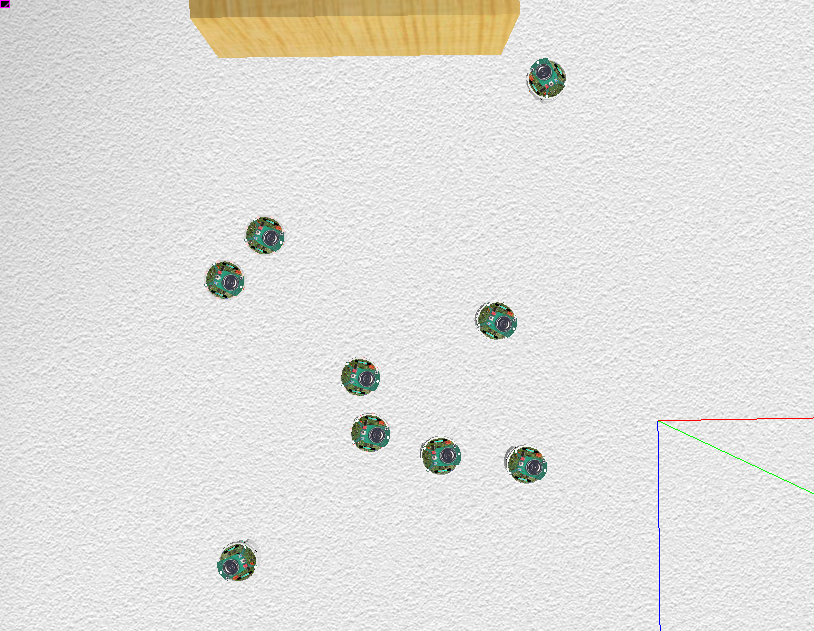
\includegraphics[width=.5\linewidth]{epuck-bees}
	\captionof{figure}{Swarm of bees vs a swarm of e-pucks}
	\label{fig:bees}
\end{figure}

Owing to the e-puck swarm's rapid movements within the swarm boundary, the most similar biological equivalent would be a swarm of bees. As can be seen from Figure \ref{fig:bees}, both systems exhibit strikingly similar behaviour. Both are homogenous groups, forming a loose collective of units. The majority of agents of both groups are oriented to the same heading, with some outliers steering toward the group. 

Through analysis of the above experiment, the question can be answered. The swarm system can be said to be exhibiting flocking and is an example of biologically inspired behaviour.
\clearpage
\subsection{Experiment 2}

\tabulinesep = 1mm
\begin{figure}[!h]
	\centering
	\begin{minipage}{.6\textwidth}
		\centering
		\begin{tabu} to .75\textwidth { | X[c] | X[c] | }
			\hline
			Run & Average time steps (32ms)\\
			\hline
			1 & 920 \\
			\hline
			2 & 380 \\
			\hline
			3 & 1459 \\
			\hline
			4 & 1873 \\
			\hline
			5 & 914 \\
			\hline
			Average & 1109 (35.488s) \\
			\hline
		\end{tabu}
		\caption{Average time steps to aggregation} 	% \caption IS ALWAYS FIRST
		\label{fig:average-time} 	% \label IS ALWAYS SECOND
	\end{minipage}
\end{figure}

In order to answer this question, the average of multiple simulation runs were made. It can be seen from Fig. \ref{fig:average-time} that the average time to aggregation is 35.488 seconds. This is in line with Fig. \ref{fig:sw5}. The wide range in average times can be explained by the randomness of movement that is inherrent in emergent systems like this one.

Though the time to aggregation is fast, this can be improved further if a higher level controller is directing the behaviour of every e-puck. However, this would not be a true, decentralised swarm system and would thus be more susceptible to errors and failure.

\clearpage

\subsection{Experiment 3}

\begin{figure}[!h]
	\centering
	\begin{minipage}{.5\textwidth}
		\centering
		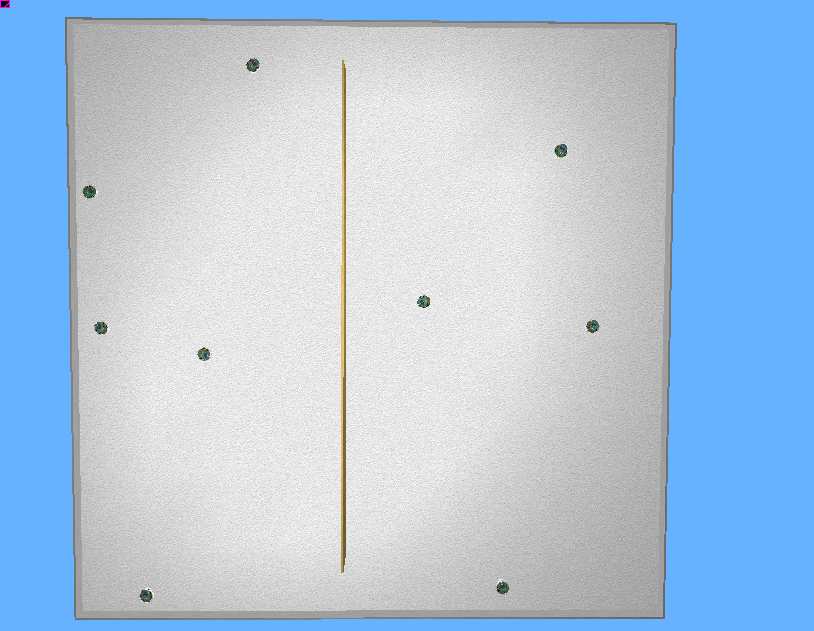
\includegraphics[width=.75\linewidth]{segregate1}
		\caption*{t = 0s}
		\label{fig:seg1}
	\end{minipage}%
	\begin{minipage}{.5\textwidth}
		\centering
		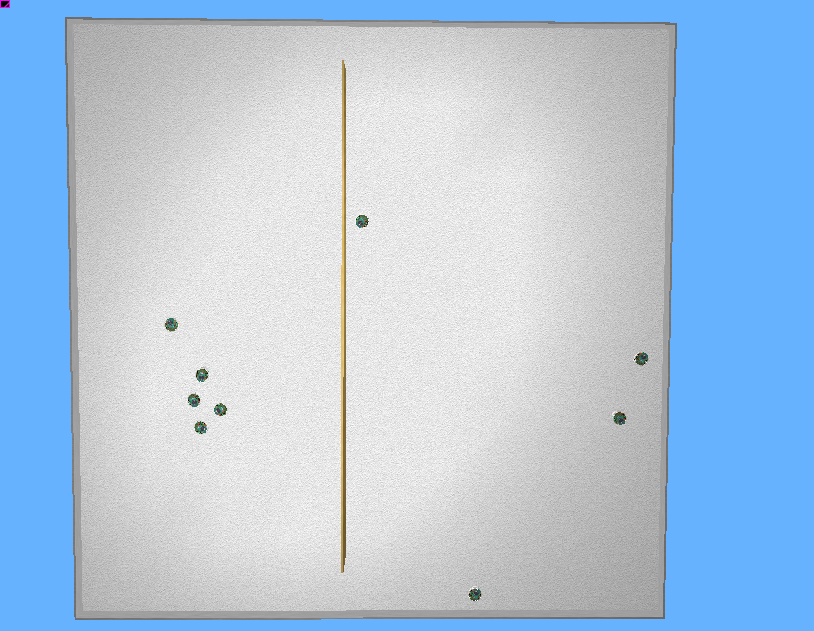
\includegraphics[width=.75\linewidth]{segregate2}
		\caption*{t = 20s}
		\label{fig:seg2}
	\end{minipage}
	\begin{minipage}{.5\textwidth}
		\centering
		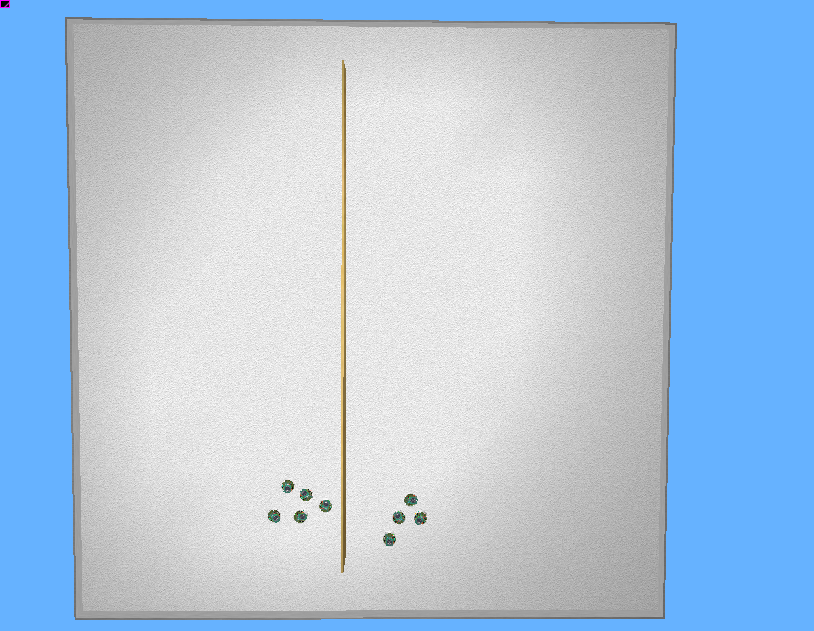
\includegraphics[width=.75\linewidth]{segregate3}
		\caption*{t = 60s}
		\label{fig:seg3}
	\end{minipage}%
	\begin{minipage}{.5\textwidth}
	\centering
	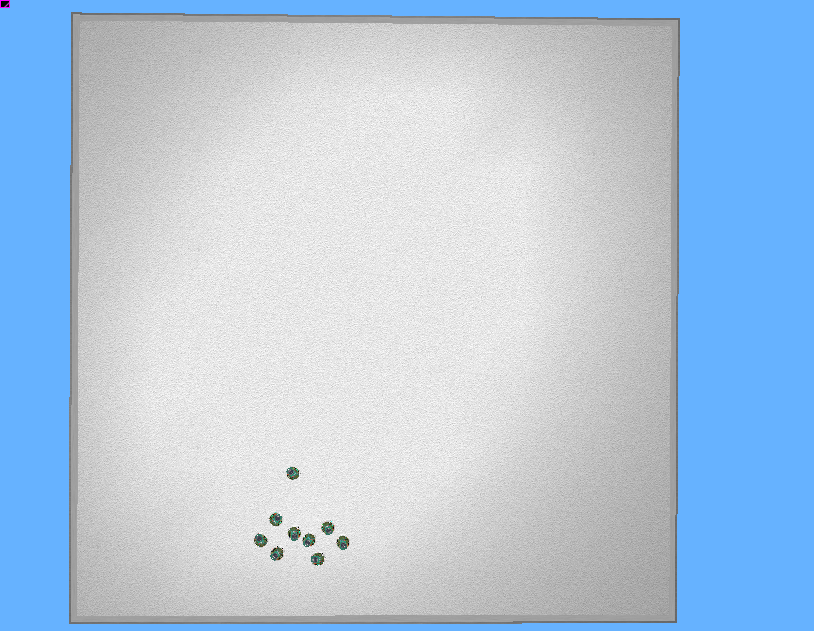
\includegraphics[width=.75\linewidth]{segregate4}
	\caption*{t = 70s}
	\label{fig:seg4}
\end{minipage}%	
	\captionof{figure}{Splinter group test}
	\label{fig:seg}
\end{figure}

Figure \ref{fig:seg} shows the segregated system over a 70 second time period. As predicted, each group on either side of the barrier are quickly able to form independent formations, though the  time taken to do this is increased due to a decrease in swarm density. Once the barrier is removed, the two groups quickly attract one another and amalgamate to form one flock.

This is due to the inherrent locality of the swarm's interactions. Each member of the swarm does not have information on the state of the entire system, thus it behaves according to what is presented to it nearby.

In addition to this, this experiment showed the ability of the swarm to operate in a different and changing environment. Again, this is due to the locality of the agent-agent interactions. This is a demonstration of how crucial the concept of locality is to a swarm's ability to cope with fault tolerance and a dynamic environment.
\clearpage

\subsection{Experiment 4}

\begin{figure}[!h]
	\centering
	\begin{minipage}{.5\textwidth}
		\centering
		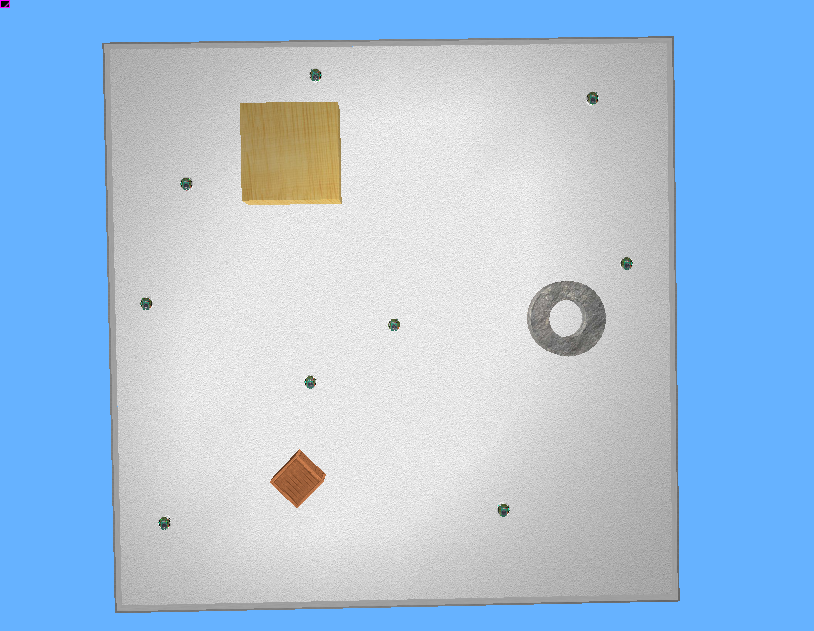
\includegraphics[width=.75\linewidth]{failure1}
		\caption*{t = 0s}
		\label{fig:sfail1}
	\end{minipage}%
	\begin{minipage}{.5\textwidth}
		\centering
		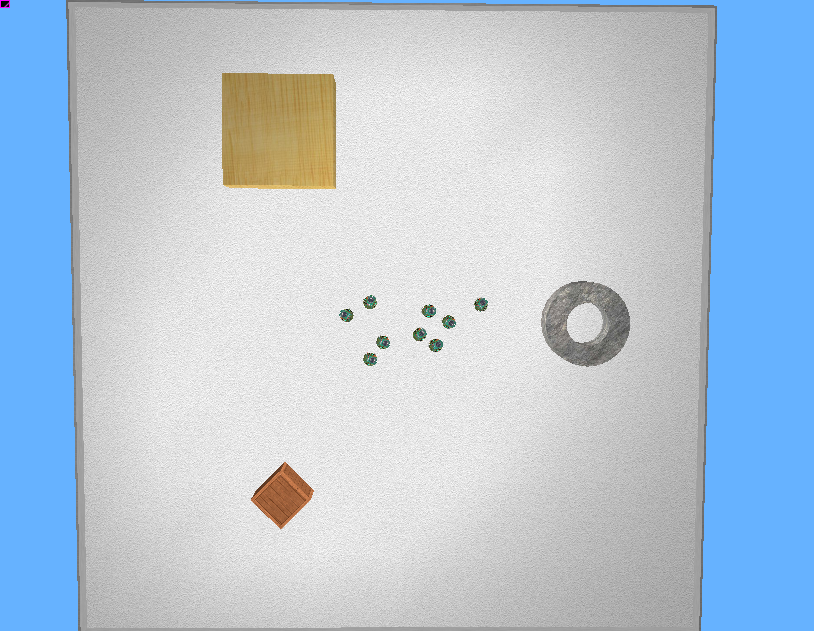
\includegraphics[width=.75\linewidth]{failure2}
		\caption*{t = 35s}
		\label{fig:fail2}
	\end{minipage}
	\begin{minipage}{.5\textwidth}
		\centering
		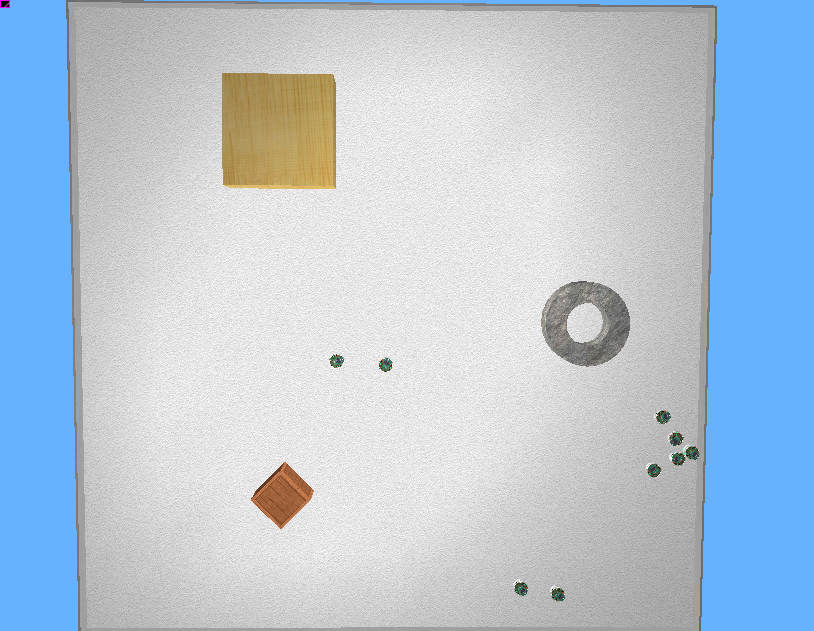
\includegraphics[width=.75\linewidth]{failure3}
		\caption*{t = 180s}
		\label{fig:fail3}
	\end{minipage}%
	\captionof{figure}{Failure test}
	\label{fig:fail}
\end{figure}

The simulation was allowed to progress until a flock had amalgamated, in this case at \(t = 35s\). After this instance, two agents were powered down (e-puck1 and e-puck4, in the center of the arena) to simulate a fatal error/fault. It can be seen in Fig. \ref{fig:fail} that over time, the system ignores these two inoperable robots and continues exhibiting flocking behaviour. 

This is because the functional agents do not receive any signals from the inoperable agents and will treat them as if they were another obstacle in the environment, something to be avoided. 

This can be validated through Fig. \ref{fig:exp4}. As can be seen, all robots bar e-puck1 and e-puck4 settle at detecting 6 robots, which is the total number of functional robots in the swarm.

\begin{sidewaysfigure}
	\centering
	\begin{minipage}{1\textwidth}
		\centering
		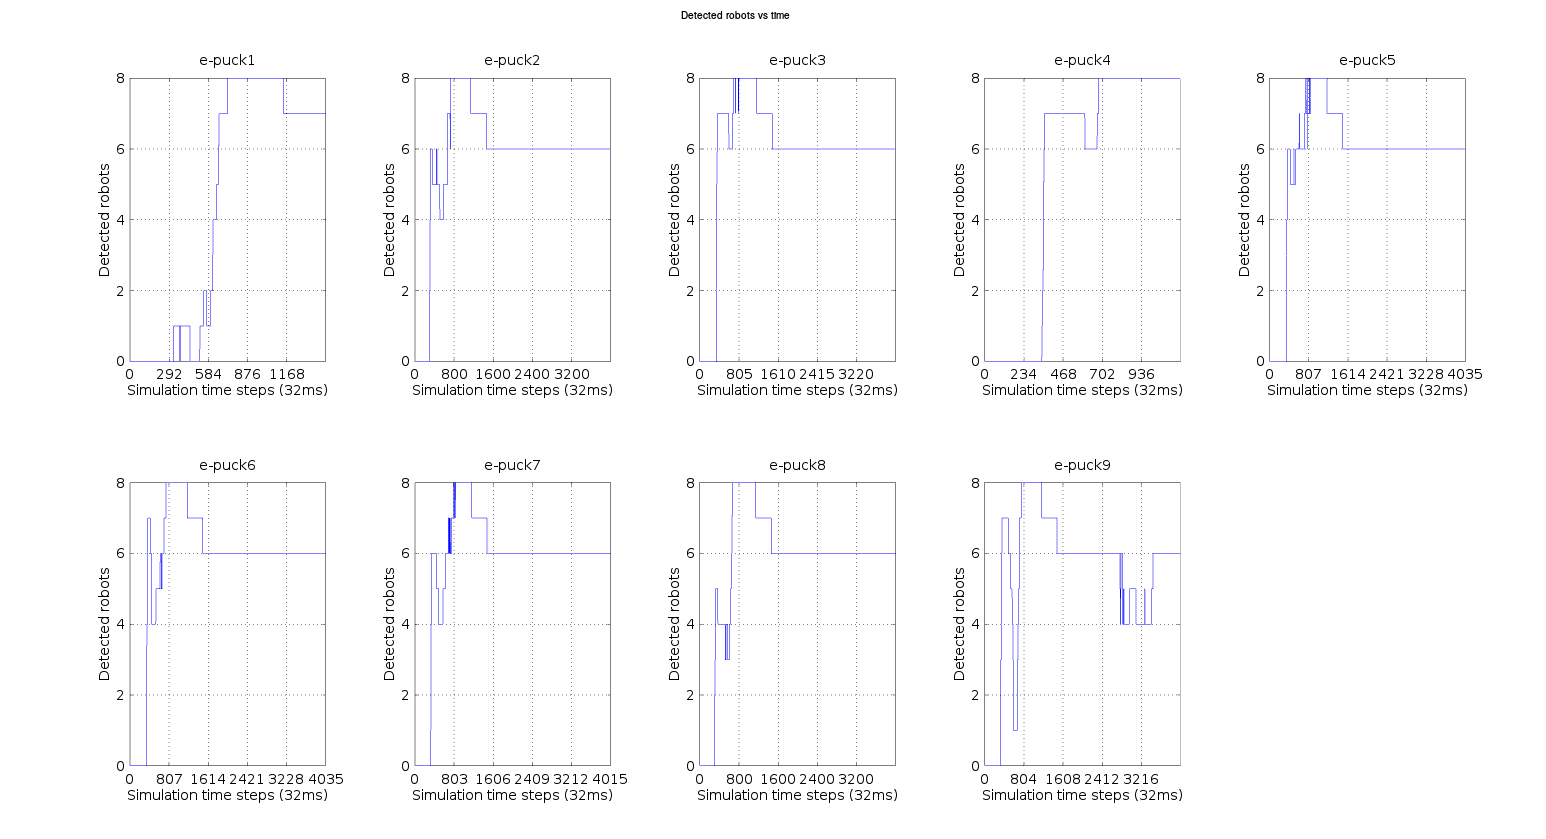
\includegraphics[width=1\linewidth]{data-failure}
		\captionof{figure}{Number of robots detected vs time}
		\label{fig:exp4}
	\end{minipage}%
\end{sidewaysfigure}
\clearpage

\subsection{Experiment 5}

\begin{figure}[!h]
	\centering
	\begin{minipage}{.5\textwidth}
		\centering
		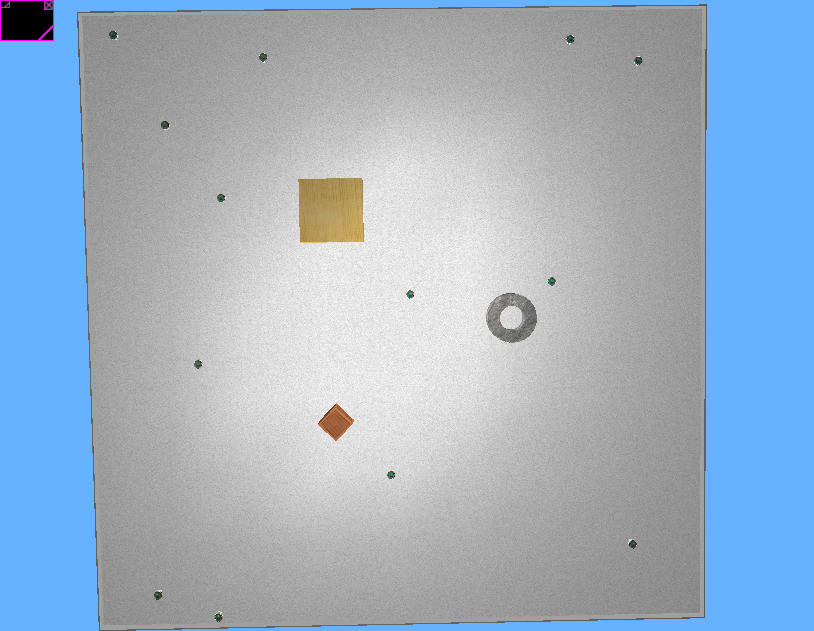
\includegraphics[width=.75\linewidth]{scalable1}
		\caption*{t = 0s}
		\label{fig:scale1}
	\end{minipage}%
	\begin{minipage}{.5\textwidth}
		\centering
		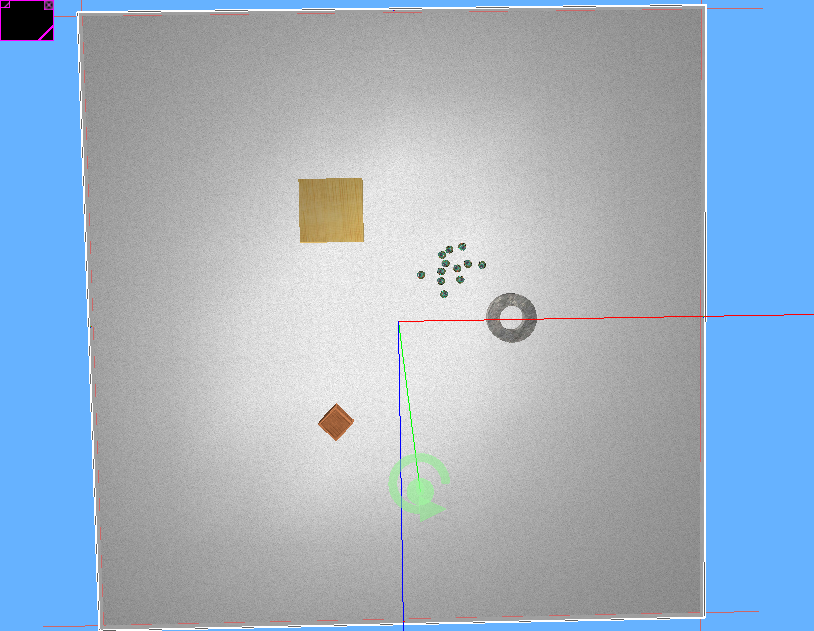
\includegraphics[width=.75\linewidth]{scalable2}
		\caption*{t = 90s}
		\label{fig:scale2}
	\end{minipage}
	\captionof{figure}{Scalability test}
	\label{fig:scale}
\end{figure}

\begin{figure}[h]
	\centering
	\begin{minipage}{1\textwidth}
		\centering
		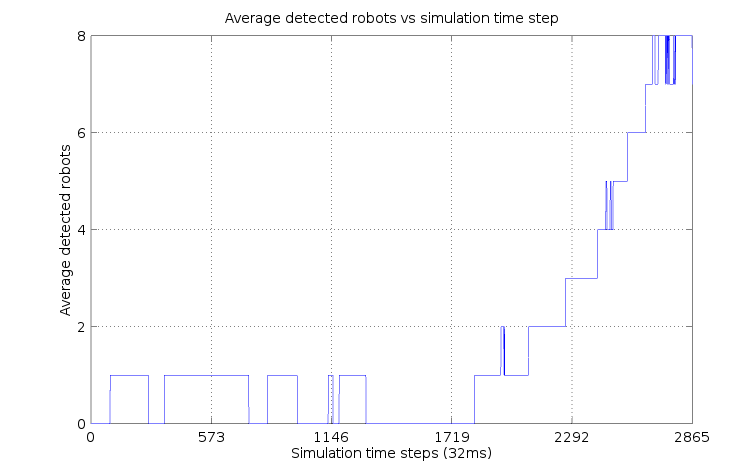
\includegraphics[width=.75\linewidth]{data-scale1}
		\captionof{figure}{Average number of detected robots}
		\label{fig:exp5}
	\end{minipage}%
\end{figure}

Finally, one of the key features of a robot swarm system is its ability to scale in size and still exhibit similar behaviour. 

Along side the swarm's ability to handle errors and faults, Experiment 4 showed how the swarm is capable of scaling \textit{down} in size and still function properly (agent count decreased from 9 to 7). This experiment aimed to shed light on the swarm's ability to scale \textit{up}.

In this case, another 3 agents were introduced to the environment (an increase of 33\%) and the simulation was executed. Shown in Fig. \ref{fig:scale} is a 90 second period of time from the beginning of the simulation. By the end, the swarm had coalesced into a similar formation as shown in previous experiments. 

Once again, this is due to the local nature of the agent-agent interactions. The individual agents do not care about the state of the agents it cannot see nor does it glean any information from a global source.

Adding extra agents to the system does increase the workload that is placed on the simulator, with the simulation running slower than previously. However, this does not effect the behaviour of the robot controller so is ignored. 